\section{Análisis del Problema}

El problema a resolver consiste en el desarrollo de una aplicación para el
manejo de un restaurante y lo que esto implica, específicamente, el manejo de 
las órdenes de los clientes, la administración de los productos y la 
generación de reportes de ventas. El desarrollo de la aplicación 
consta de tres grandes aspectos: la interfaz gráfica, la base de datos y 
la lógica de negocio.

Con respecto a la interfaz gráfica, se debe de desarrollar de forma que 
cumpla con los requerimientos establecidos en la especificación del proyecto,
a continuación se listan los requerimientos más importantes:

\begin{itemize}
    \item Ofrecer una vista para el manejo de inventario, en la cual se 
    puedan agregar, modificar y eliminar productos.
    \item Ofrecer una vista para el manejo de platos existentes, en la cual
    se puedan agregar, modificar y eliminar platos, los cuales son creados 
    a partir de la combinación de productos.
    \item Ofrecer una vista para el manejo de órdenes, en la cual se puedan 
    agregar, modificar y eliminar órdenes, las cuales son creadas a partir
    de un número de mesa, la cantidad de comensales, el tipo de orden, si es 
    por mesa o por persona, y los platos que se ordenaron, entre los cuales 
    existen platos del menú predefinido y platos personalizados (creados a 
    partir de la combinación de productos, tomando en cuenta las restricciones 
    del cliente).
    \item Ofrecer una vista que permita visualizar estadísticas de ventas, 
    entre las cuales se desea conocer información significativa para el 
    restaurante, con respecto a las ventas, el menú y productos.
    \item Ofrecer una vista para visualizar las facturas de las órdenes, donde 
    se muestre la información de la orden, el total de la orden y el 
    detalle de la orden.
\end{itemize}

Con respecto a la base de datos, se debe de desarrollar de forma que sea capaz
de almacenar toda la información necesaria para el correcto funcionamiento de 
la aplicación.

Con respecto a la lógica de negocio, se debe de desarrollar de forma que 
cumpla con los requerimientos establecidos en la especificación del proyecto, 
cabe destacar que en la lógica de negocio se deben de implementar al menos 
tres patrones de diseño, a continuación se listan los requerimientos más 
importantes:

\begin{itemize}
    \item Permitir la creación de platos personalizados, a partir de la 
    combinación de productos, tomando en cuenta las restricciones del cliente, 
    estos platos deben de ser generados utilizando el paradigma de programación
    lógica, por medio de Prolog.
    \item Manipular y ofrecer toda la información necesaria para el correcto 
    funcionamiento de la interfaz gráfica, por medio de un lenjuage de 
    programación orientado a objetos. 
\end{itemize}

De esta forma, se puede concluir que el problema a resolver es un problema 
de programación orientada a objetos y programación lógica, por lo que se 
debe de utilizar un lenguaje de programación que permita la implementación 
de ambos paradigmas, a continuación en la siguiente sección se discutirán 
las tecnologías utilizadas para el desarrollo de la aplicación.

\section{Solución del Problema}

Para la solución del problema planteado, se decidió utilizar el lenguaje de 
programación Python, se tomó esta decisión debido a que Python es un
lenguaje de programación multiparadigma, el cual permite la implementación 
del paradigma de programación orientada a objetos, además de contar 
con una amplia variedad de librerías que facilitan el desarrollo de
la aplicación y la integración con otras tecnologías y herramientas, 
en adición, Python es un lenguaje de programación interpretado, lo cual 
facilitará la ejecución de la aplicación en diferentes sistemas operativos.

Para el desarrollo de la interfaz gráfica, se decidió optar por una 
solución un poco distinta a lo establecido en la especificación del 
proyecto, sin embargo, a criterio del equipo de desarrollo, esta solución 
dará una mejor experiencia de usuario, además de que facilitará el 
desarrollo de la aplicación, esta solución consiste en el desarrollo de 
una aplicación web, de esta forma, se implementa el primer patrón de diseño, 
el patrón de diseño Modelo-Vista-Controlador (MVC), el cual permite separar 
la lógica de negocio de la interfaz gráfica, de esta forma, se implementa 
el primer patrón de diseño, el patrón de diseño Modelo-Vista-Controlador 
(MVC), el cual permite separar la lógica de negocio de la interfaz gráfica.

Para el desarrollo de la base de datos, se decidió utilizar SQLite, debido 
a que es un sistema de gestión de bases de datos relacional, el cual 
permite el almacenamiento de toda la información necesaria para el correcto 
funcionamiento de la aplicación, además de que es un sistema de gestión de 
bases de datos ligero, el cual no requiere de un servidor para su 
funcionamiento, lo cual facilita la implementación de la aplicación.

Para el desarrollo de la lógica de negocio, como se mencionó anteriormente, 
se decidió utilizar el lenguaje de programación Python, al estar utilizando 
el patrón de diseño Modelo-Vista-Controlador (MVC), las conexiones a la base de
datos, con Prolog y con la interfaz gráfica, se encuentran en el controlador, \
por otro lado, la vista se encuentra en la interfaz gráfica, y el modelo se
encuentra tanto en la base de datos como en la lógica de negocio para su
correcto funcionamiento.

A continuación se hará una descripción de cada uno de las soluciones 
para los requerimientos establecidos en el análisis del problema.

\subsection{Interfaz Gráfica}

Para el desarrollo de la interfaz gráfica, se decidió utilizar el framework 
Vue.js, el cual es un framework progresivo para el desarrollo de interfaces
de usuario, el cual permite la creación de interfaces de usuario de forma 
modular \cite{vuejs}, se centra en la capa de vista de una aplicación web y se
utiliza para crear interfaces de usuario dinámicas y atractivas. Además, 
se utiliza Bootstrap y Element Plus para el desarrollo de la interfaz gráfica, 
frameworks de CSS y JavaScript, los cuales permiten el desarrollo de interfaces
de usuario de forma rápida y sencilla.

\subsubsection{Inventario}

Para el manejo de inventario, se decidió implementar una vista que permita 
agregar, modificar y eliminar productos, para esto, se creó un formulario 
que permite agregar un producto, el cual contiene los siguientes campos: 
nombre, calorias, precio, cantidad y tipo, ver figura \ref{fig:inventory_add},
además, se creó una vista que permite visualizar todos los productos
existentes, en esta vista se puede modificar y eliminar un producto, además de
que se puede acceder a la vista de agregar un producto, ver figura
\ref{fig:inventory}, en esta vista existe la opción de filtrar los productos 
por nombre y tipo.

\begin{figure}[H]
    \centering
    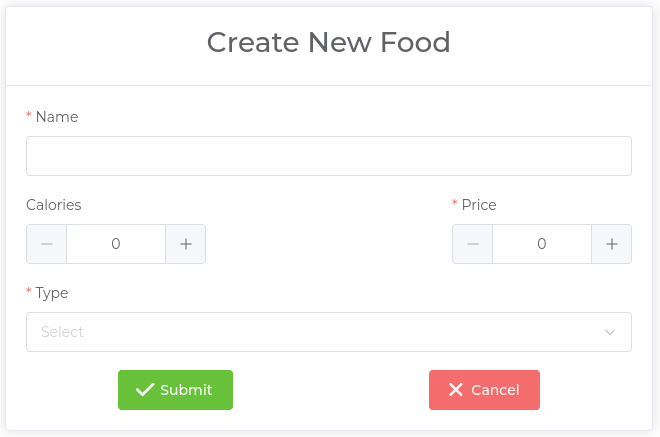
\includegraphics[width=0.4\textwidth]{assets/inventory_add.png}
    \caption{Vista de agregar un producto}
    \label{fig:inventory_add}
\end{figure}

\begin{figure}[H]
    \centering
    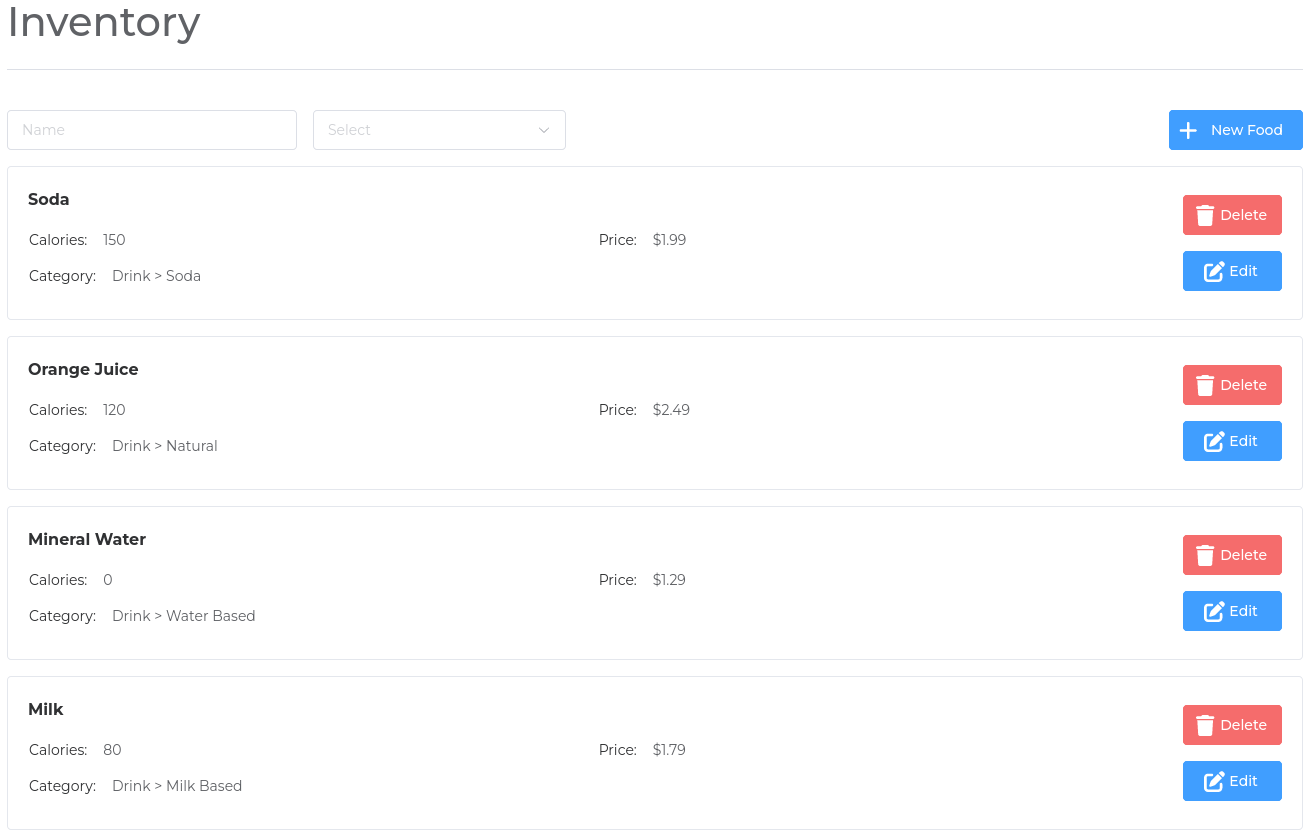
\includegraphics[width=0.4\textwidth]{assets/inventory.png}
    \caption{Vista de Inventario}
    \label{fig:inventory}
\end{figure}

\subsubsection{Platos}

Para el manejo de platos, se decidió implementar una vista que permita 
agregar, modificar y eliminar platos, para esto, se creó un formulario 
que permite agregar un plato, el cual contiene los siguientes campos: 
nombre y los productos que lo componen, ver figura \ref{fig:dishes_add},
además, se creó una vista que permite visualizar todos los platos 
existentes, en esta vista se puede modificar y eliminar un plato, además de 
que se puede acceder a la vista de agregar un plato, ver figura 
\ref{fig:dishes}, en esta vista existe la opción de filtrar los platos por 
nombre.

\begin{figure}[H]
    \centering
    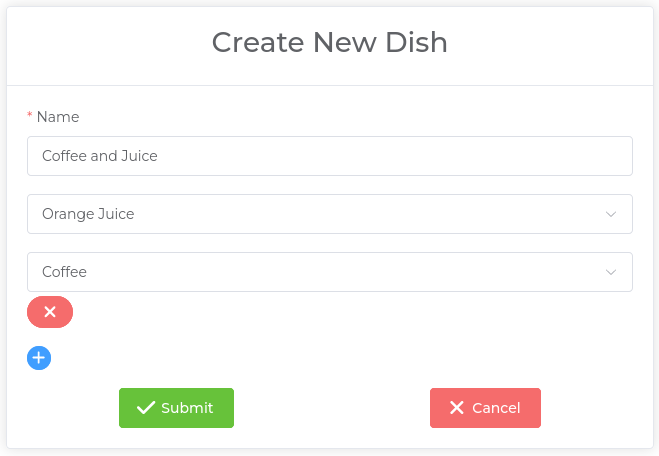
\includegraphics[width=0.4\textwidth]{assets/dishes_add.png}
    \caption{Vista de agregar un plato}
    \label{fig:dishes_add}
\end{figure}

\begin{figure}[H]
    \centering
    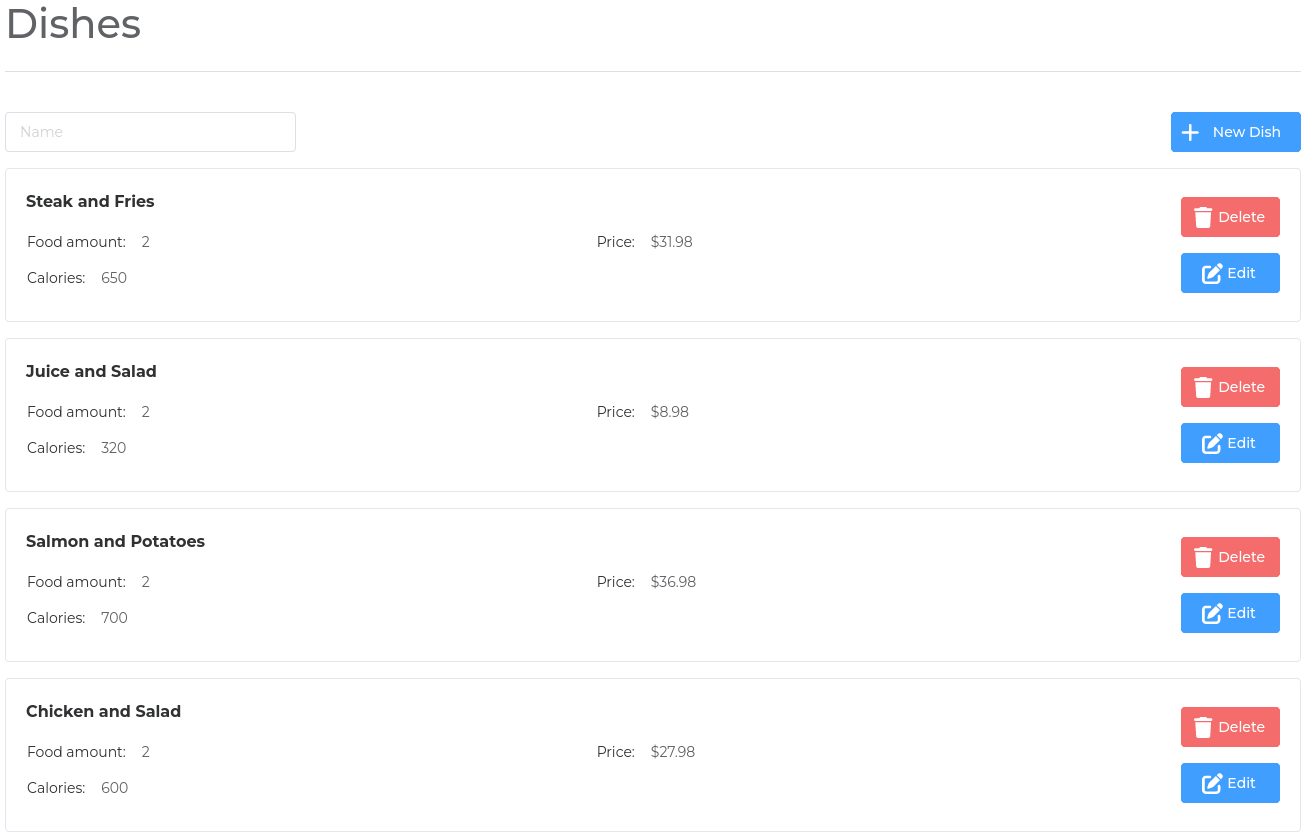
\includegraphics[width=0.4\textwidth]{assets/dishes.png}
    \caption{Vista de Platos}
    \label{fig:dishes}
\end{figure}

\subsubsection{Órdenes}

\subsubsection{Estadísticas}

En esta vista se logra visualizar información significativa para el 
restaurante, con respecto a las ventas, el menú y productos, se puede 
visualizar el total de ventas, el total productos en inventario, el total 
de platos en el menú, el total de ordenes, un gráfico lineal con la 
cantidad de ventas y ganancias por día, un gráfico de barras con los  
productos más vendidos y un gráfico de barras con los platos más vendidos, 
ver figura \ref{fig:statistics}.

\begin{figure}[H]
    \centering
    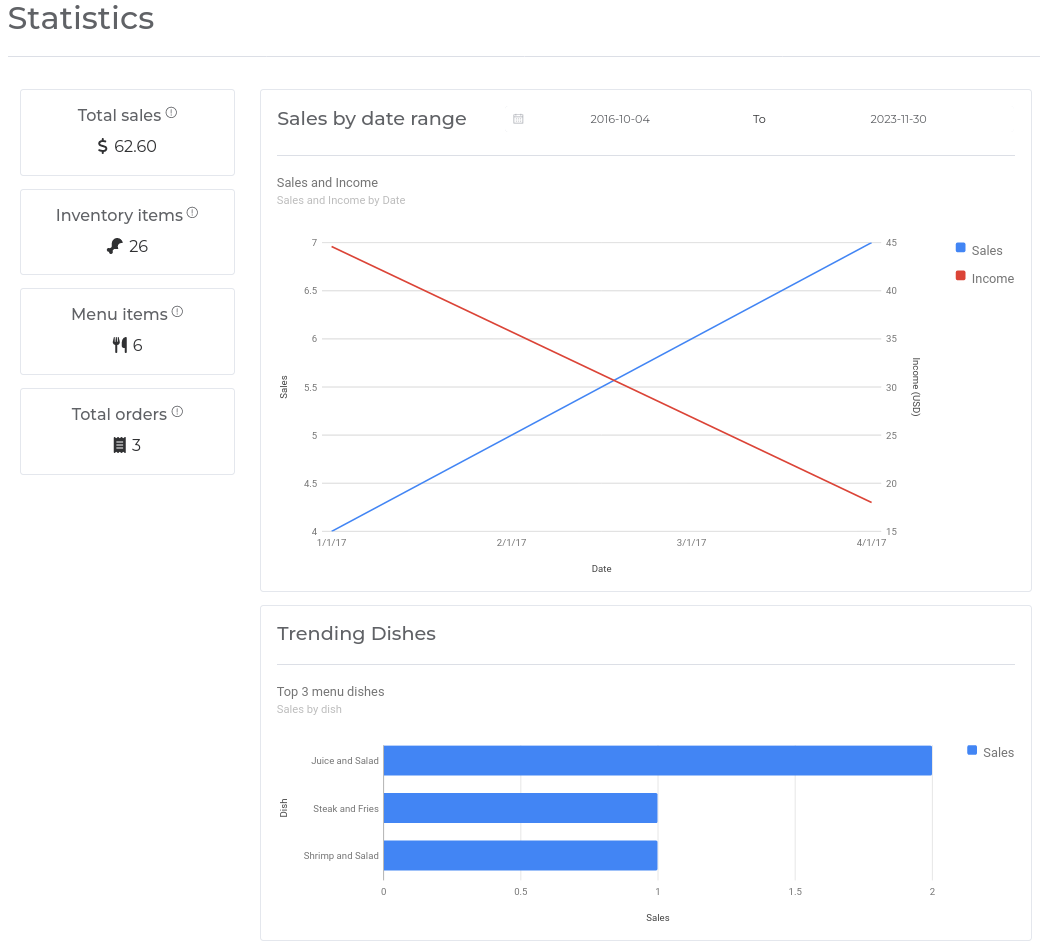
\includegraphics[width=0.4\textwidth]{assets/statistics.png}
    \caption{Vista de Estadísticas}
    \label{fig:statistics}
\end{figure}

\subsubsection{Facturas}

Para el manejo de facturas, se decidió implementar una vista que permita 
visualizar las facturas de las órdenes, donde se muestre la información de 
la orden, el total de la orden y el detalle de la orden, ver figura 
\ref{fig:invoices}, además de poder filtrar las facturas por tipo de pago, 
total de la orden y fecha.

\begin{figure}[H]
    \centering
    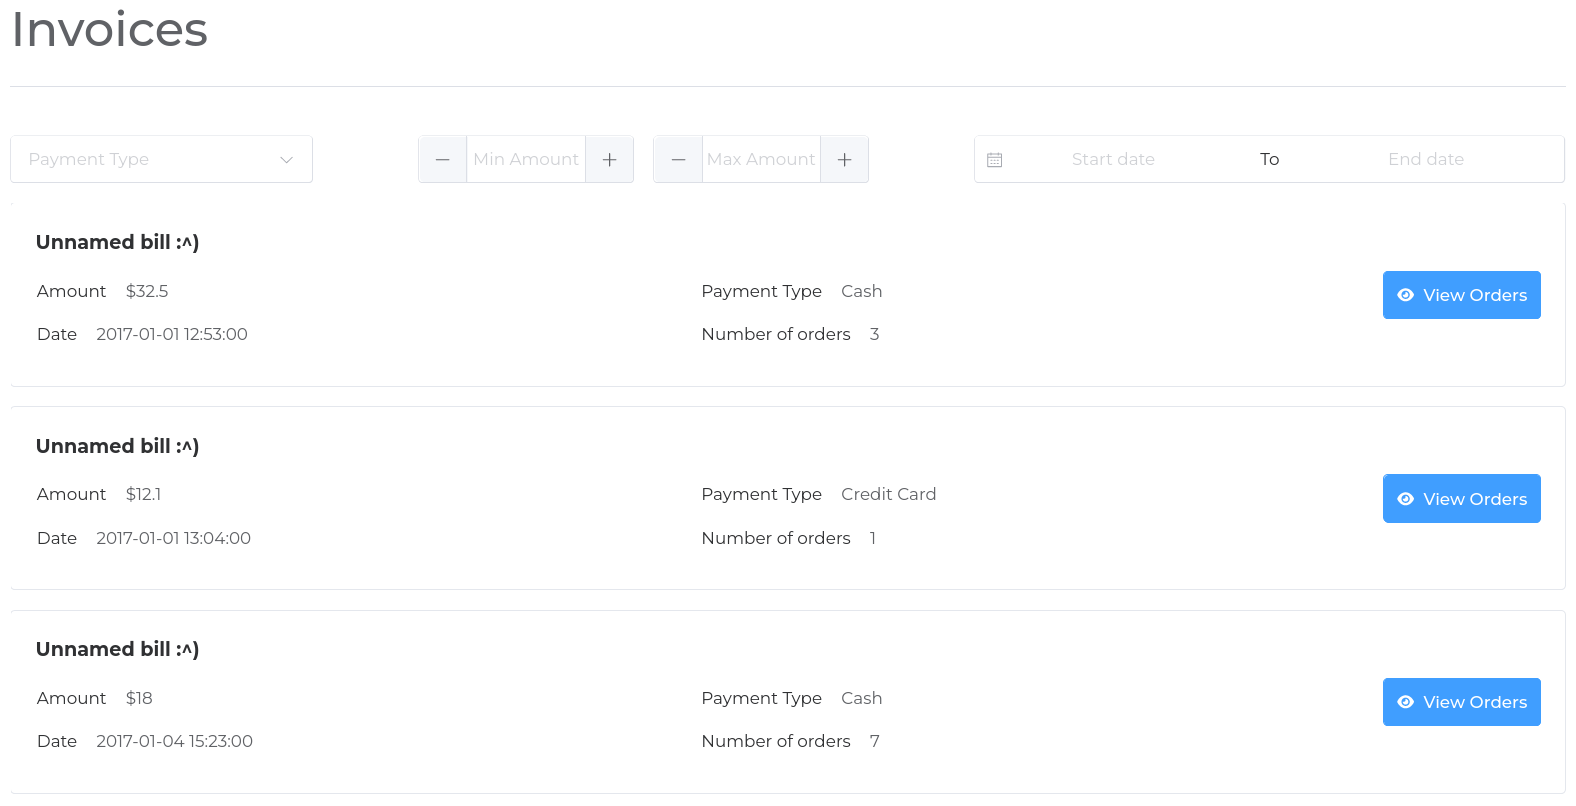
\includegraphics[width=0.4\textwidth]{assets/invoices.png}
    \caption{Vista de Facturas}
    \label{fig:invoices}
\end{figure}

\subsection{Base de Datos}

Tal y como se mencionó anteriormente, para el desarrollo de la base de datos, 
se decidió utilizar SQLite, en la figura \ref{fig:database} se puede 
observar el diagrama de la base de datos, en el cual se puede observar 
que la base de datos cuenta con tablas para almacenar la información de 
los productos, los platos, las órdenes, los detalles de las órdenes y 
las facturas de las órdenes, además de que se cuenta con tablas para 
el manejo de estadísticas, las cuales se actualizan por medio de 
triggers, los cuales se ejecutan cuando se inserta, modifica o elimina 
de la base de datos.

\begin{figure}[H]
    \centering
    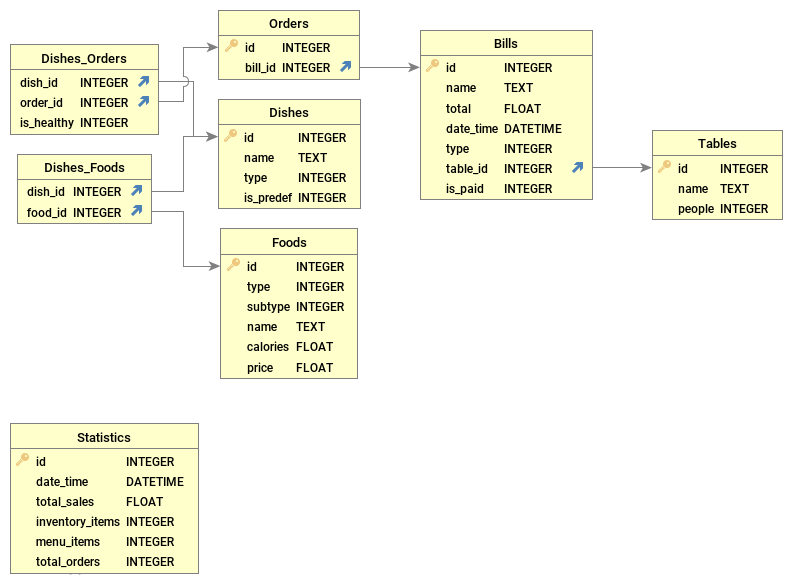
\includegraphics[width=0.4\textwidth]{assets/database.png}
    \caption{Diagrama de la base de datos}
    \label{fig:database}
\end{figure}

\subsection{Lógica de Negocio}

Por último, para el desarrollo de la lógica de negocio, se utilizó el 
lenguaje de programación Python para conectar la base de datos, 
la interfaz gráfica y Prolog entre sí. Para la conexión con la base de 
datos se utilizó el módulo sqlite3 y el patrón de diseño Singleton, de modo 
que se pueda acceder a la base de datos desde cualquier parte de la 
aplicación. Para la conexión con Prolog se utilizó el módulo swiplserver, 
el cual permite la conexión con Prolog por medio de un servidor, de esta 
forma, se puede ejecutar código Prolog desde Python, además de que se 
utilizó el patrón de diseño Singleton, de modo que se pueda acceder a 
Prolog desde cualquier parte de la aplicación. Para la conexión con la 
interfaz gráfica se utilizó el módulo flask, el cual permite la creación 
de una aplicación web. Para el modelado de los datos se utilizó el 
patrón de diseño Builder, de esta forma se obtienen los datos de la base 
a través del controlador, se modelan y se envían a la vista, para que 
sean mostrados al usuario.

Por el lado de Prolog, se crearón reglas para la creación de platos 
a partir de criterios establecidos por el cliente, de modo que 
se generen todas las combinaciones posibles de productos, siempre y
cuando cumplan con los criterios establecidos por el cliente.
